% Options for packages loaded elsewhere
\PassOptionsToPackage{unicode}{hyperref}
\PassOptionsToPackage{hyphens}{url}
%
\documentclass[
  french,
]{article}
\usepackage{lmodern}
\usepackage{amssymb,amsmath}
\usepackage{ifxetex,ifluatex}
\ifnum 0\ifxetex 1\fi\ifluatex 1\fi=0 % if pdftex
  \usepackage[T1]{fontenc}
  \usepackage[utf8]{inputenc}
  \usepackage{textcomp} % provide euro and other symbols
\else % if luatex or xetex
  \usepackage{unicode-math}
  \defaultfontfeatures{Scale=MatchLowercase}
  \defaultfontfeatures[\rmfamily]{Ligatures=TeX,Scale=1}
\fi
% Use upquote if available, for straight quotes in verbatim environments
\IfFileExists{upquote.sty}{\usepackage{upquote}}{}
\IfFileExists{microtype.sty}{% use microtype if available
  \usepackage[]{microtype}
  \UseMicrotypeSet[protrusion]{basicmath} % disable protrusion for tt fonts
}{}
\makeatletter
\@ifundefined{KOMAClassName}{% if non-KOMA class
  \IfFileExists{parskip.sty}{%
    \usepackage{parskip}
  }{% else
    \setlength{\parindent}{0pt}
    \setlength{\parskip}{6pt plus 2pt minus 1pt}}
}{% if KOMA class
  \KOMAoptions{parskip=half}}
\makeatother
\usepackage{xcolor}
\IfFileExists{xurl.sty}{\usepackage{xurl}}{} % add URL line breaks if available
\IfFileExists{bookmark.sty}{\usepackage{bookmark}}{\usepackage{hyperref}}
\hypersetup{
  pdftitle={Contrôle Optimale},
  pdfauthor={Rand ASSWAD A l'attention de Mme. Rachida AL MASSOUDI},
  pdflang={fr-FR},
  hidelinks,
  pdfcreator={LaTeX via pandoc}}
\urlstyle{same} % disable monospaced font for URLs
\usepackage[margin=1in]{geometry}
\usepackage{color}
\usepackage{fancyvrb}
\newcommand{\VerbBar}{|}
\newcommand{\VERB}{\Verb[commandchars=\\\{\}]}
\DefineVerbatimEnvironment{Highlighting}{Verbatim}{commandchars=\\\{\}}
% Add ',fontsize=\small' for more characters per line
\usepackage{framed}
\definecolor{shadecolor}{RGB}{248,248,248}
\newenvironment{Shaded}{\begin{snugshade}}{\end{snugshade}}
\newcommand{\AlertTok}[1]{\textcolor[rgb]{0.94,0.16,0.16}{#1}}
\newcommand{\AnnotationTok}[1]{\textcolor[rgb]{0.56,0.35,0.01}{\textbf{\textit{#1}}}}
\newcommand{\AttributeTok}[1]{\textcolor[rgb]{0.77,0.63,0.00}{#1}}
\newcommand{\BaseNTok}[1]{\textcolor[rgb]{0.00,0.00,0.81}{#1}}
\newcommand{\BuiltInTok}[1]{#1}
\newcommand{\CharTok}[1]{\textcolor[rgb]{0.31,0.60,0.02}{#1}}
\newcommand{\CommentTok}[1]{\textcolor[rgb]{0.56,0.35,0.01}{\textit{#1}}}
\newcommand{\CommentVarTok}[1]{\textcolor[rgb]{0.56,0.35,0.01}{\textbf{\textit{#1}}}}
\newcommand{\ConstantTok}[1]{\textcolor[rgb]{0.00,0.00,0.00}{#1}}
\newcommand{\ControlFlowTok}[1]{\textcolor[rgb]{0.13,0.29,0.53}{\textbf{#1}}}
\newcommand{\DataTypeTok}[1]{\textcolor[rgb]{0.13,0.29,0.53}{#1}}
\newcommand{\DecValTok}[1]{\textcolor[rgb]{0.00,0.00,0.81}{#1}}
\newcommand{\DocumentationTok}[1]{\textcolor[rgb]{0.56,0.35,0.01}{\textbf{\textit{#1}}}}
\newcommand{\ErrorTok}[1]{\textcolor[rgb]{0.64,0.00,0.00}{\textbf{#1}}}
\newcommand{\ExtensionTok}[1]{#1}
\newcommand{\FloatTok}[1]{\textcolor[rgb]{0.00,0.00,0.81}{#1}}
\newcommand{\FunctionTok}[1]{\textcolor[rgb]{0.00,0.00,0.00}{#1}}
\newcommand{\ImportTok}[1]{#1}
\newcommand{\InformationTok}[1]{\textcolor[rgb]{0.56,0.35,0.01}{\textbf{\textit{#1}}}}
\newcommand{\KeywordTok}[1]{\textcolor[rgb]{0.13,0.29,0.53}{\textbf{#1}}}
\newcommand{\NormalTok}[1]{#1}
\newcommand{\OperatorTok}[1]{\textcolor[rgb]{0.81,0.36,0.00}{\textbf{#1}}}
\newcommand{\OtherTok}[1]{\textcolor[rgb]{0.56,0.35,0.01}{#1}}
\newcommand{\PreprocessorTok}[1]{\textcolor[rgb]{0.56,0.35,0.01}{\textit{#1}}}
\newcommand{\RegionMarkerTok}[1]{#1}
\newcommand{\SpecialCharTok}[1]{\textcolor[rgb]{0.00,0.00,0.00}{#1}}
\newcommand{\SpecialStringTok}[1]{\textcolor[rgb]{0.31,0.60,0.02}{#1}}
\newcommand{\StringTok}[1]{\textcolor[rgb]{0.31,0.60,0.02}{#1}}
\newcommand{\VariableTok}[1]{\textcolor[rgb]{0.00,0.00,0.00}{#1}}
\newcommand{\VerbatimStringTok}[1]{\textcolor[rgb]{0.31,0.60,0.02}{#1}}
\newcommand{\WarningTok}[1]{\textcolor[rgb]{0.56,0.35,0.01}{\textbf{\textit{#1}}}}
\usepackage{longtable,booktabs}
% Correct order of tables after \paragraph or \subparagraph
\usepackage{etoolbox}
\makeatletter
\patchcmd\longtable{\par}{\if@noskipsec\mbox{}\fi\par}{}{}
\makeatother
% Allow footnotes in longtable head/foot
\IfFileExists{footnotehyper.sty}{\usepackage{footnotehyper}}{\usepackage{footnote}}
\makesavenoteenv{longtable}
\usepackage{graphicx}
\makeatletter
\def\maxwidth{\ifdim\Gin@nat@width>\linewidth\linewidth\else\Gin@nat@width\fi}
\def\maxheight{\ifdim\Gin@nat@height>\textheight\textheight\else\Gin@nat@height\fi}
\makeatother
% Scale images if necessary, so that they will not overflow the page
% margins by default, and it is still possible to overwrite the defaults
% using explicit options in \includegraphics[width, height, ...]{}
\setkeys{Gin}{width=\maxwidth,height=\maxheight,keepaspectratio}
% Set default figure placement to htbp
\makeatletter
\def\fps@figure{htbp}
\makeatother
\setlength{\emergencystretch}{3em} % prevent overfull lines
\providecommand{\tightlist}{%
  \setlength{\itemsep}{0pt}\setlength{\parskip}{0pt}}
\setcounter{secnumdepth}{5}
\geometry{paper=a4paper, top=2cm, bottom=2cm, left=1cm, right=1cm}
\usepackage[defaultlines=10,all]{nowidow}
\usepackage{float}
\usepackage[justification=centering]{caption}

% force babel to use default item labels
%\frenchbsetup{StandardItemLabels=true}

% tables
\usepackage{boldline} % provides V{n} and \hlineB{n}
\usepackage{makecell} % for line breaks inside cell
\usepackage{multirow} % for multirow cells
\newcommand{\state}[1]{{$\begin{matrix}#1\end{matrix}$}}

% math
%\usepackage{amsmath}
%\usepackage{amsthm,amssymb,amsfonts,amscd}
\usepackage{mathtools}
\mathtoolsset{showonlyrefs}
%\usepackage{centernot}

%\DeclareMathOperator*{\argmax}{argmax}
%\DeclareMathOperator*{\argmin}{argmin}


\makeatletter

\usepackage{fancyhdr}
\pagestyle{fancy}
\lhead{\@title}
\rhead{Rand ASSWAD}

\usepackage{pmboxdraw} % for tree chars encoding

\renewcommand{\fps@figure}{H}

\AtBeginDocument{\let\maketitle\relax}

%%%%%%%%%%%%%%%% COVER

\setlength{\parindent}{0cm}
\setlength{\parskip}{1ex plus 0.5ex minus 0.2ex}
\newcommand{\hsp}{\hspace{20pt}}
\newcommand{\HRule}{\rule{\linewidth}{0.5mm}}
\ifxetex
  % Load polyglossia as late as possible: uses bidi with RTL langages (e.g. Hebrew, Arabic)
  \usepackage{polyglossia}
  \setmainlanguage[]{french}
\else
  \usepackage[shorthands=off,main=french]{babel}
\fi

\title{Contrôle Optimale}
\author{Rand ASSWAD
A l'attention de Mme. Rachida AL MASSOUDI}
\date{}

\begin{document}
\maketitle

\begin{titlepage}
    \begin{sffamily}
        \begin{center}
            
\includegraphics[width=0.8\textwidth]{img/logo}\\[2cm]

            \textsc{\huge mini-projet complémentaire}\\[1cm]

            % Title
            \HRule \\[0.4cm]
            {\huge \bfseries \@title \\[0.4cm]}
            \HRule \\[1.5cm]

            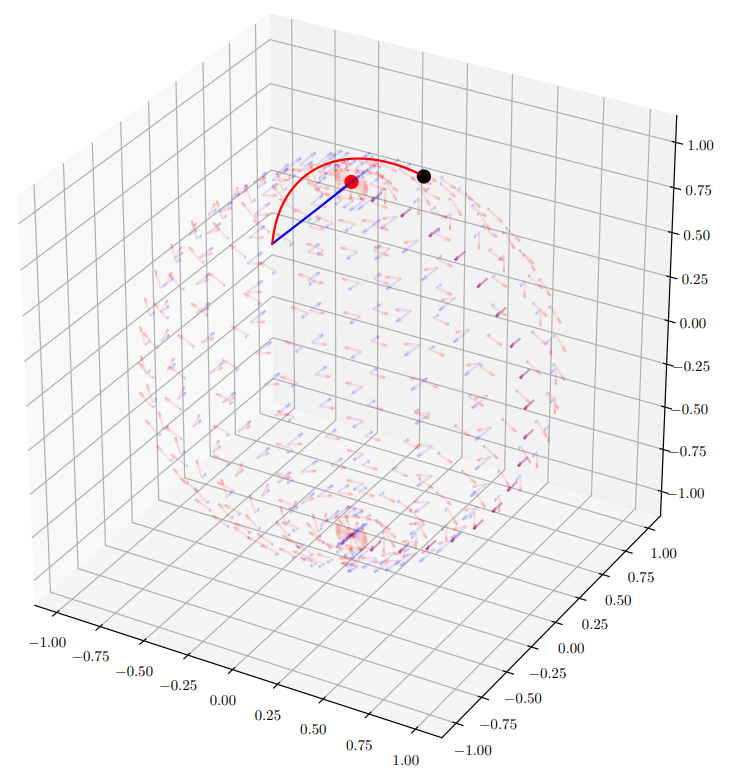
\includegraphics[width=.5\textwidth]{img/cover_img}~\\[2cm]

            % Author and supervisor
            \begin{minipage}{0.4\textwidth}
            \begin{flushleft} \large
                Rand ASSWAD\\
                Département Génie Mathématique
            \end{flushleft}
            \end{minipage}
            \begin{minipage}{0.4\textwidth}
            \begin{flushright} \large
                \emph{A l'attention de :}\\
                Mme. Rachida AL ASSOUDI
            \end{flushright}
            \end{minipage}

            \vfill
            % Bottom of the page
            {\large \@date}
        \end{center}
    \end{sffamily}
\end{titlepage}
\makeatother

\def\R{\mathbb{R}}
\def\C{\mathbb{C}}

\def\L{\mathcal{L}}
\def\U{\mathcal{U}}
\newcommand{\laplace}[1]{\L^{-1}\pp{#1}}

\def\Rnn{\R^{n\times n}}

\def\ga{\gamma}
\def\eps{\varepsilon}

\def\x{x(t)}
\def\xd{\dot{x}(t)}
\def\u{u(t)}
\def\xt{\tilde{x}}
\def\xtd{\dot{\tilde{x}}}
\def\xtopt{\tilde{x}^*}
\def\Ht{\tilde{H}}
\def\ft{\tilde{f}}

\def\dt{\mathrm{d}t}
\def\ds{\mathrm{d}s}
\newcommand{\diff}[1]{\frac{\mathrm{d}}{\dt}\pp{#1}}
\newcommand{\dif}[2]{\frac{\mathrm{d}}{\mathrm{d}#2}\pp{#1}}
\newcommand{\pd}[2]{\frac{\partial#1}{\partial#2}}

\def\sgn{\mathrm{sgn}}
\newcommand{\argmin}{\mathop{\mathrm{argmin}}}
\newcommand{\argmax}{\mathop{\mathrm{argmax}}}

\newcommand{\cas}[1]{\begin{cases}#1\end{cases}}
\newcommand{\mat}[1]{\begin{matrix}#1\end{matrix}}
\newcommand{\pmat}[1]{\begin{pmatrix}#1\end{pmatrix}}
\newcommand{\bmat}[1]{\begin{bmatrix}#1\end{bmatrix}}
\newcommand{\Bmat}[1]{\begin{Bmatrix}#1\end{Bmatrix}}

\renewcommand{\Im}{\mathrm{Im}}

\newcommand{\sset}[1]{\left\{#1\right\}}
\newcommand{\pp}[1]{\left(#1\right)}

\newcommand{\vset}[2]{\sset{#1\left\lvert\mat{#2}\right.}}

\newcommand{\norm}[1]{\left\lVert#1\right\rVert}
\newcommand{\abs}[1]{\left\lvert#1\right\rvert}
\newcommand{\dotp}[2]{\left\langle#1{,}#2\right\rangle}

\newcommand{\qtext}[1]{\quad\text{#1}\quad}
\newcommand{\qou}{\quad\mathrm{o\grave{u}}\quad}

\newcommand{\transp}[1]{{#1}^{\top}}

Dans ce mini-projet on va étudier un système de contrôle.
On trouvera ensuite les commandes qui permettent d'aller
d'un état à l'autre du système de façon optimale
par rapport à un critère donné suivant les méthodes
étudiés en cours.

\hypertarget{systuxe8me-de-contruxf4le}{%
\section{Système de contrôle}\label{systuxe8me-de-contruxf4le}}

Un système de contrôle est un système dont l'état à l'instant \(t\)
est décrit par \(n\) variables \(x_1,\ldots,x_n\). On définit le vecteur d'état
du système \(x(t)=\left(x_1(t),\ldots,x_n(t)\right)\in\mathbb{R}^n\).

On dispose de \(m\) variables de contrôle \(u_1,\ldots,u_m\) définissant la commande
appliquée à l'instant \(t\) par le vecteur \(u(t)=\left(u_1(t),\ldots,u_m(t)\right)\in\mathbb{R}^m\).

L'évolution du système est décrit par son \textbf{équation d'état}.
\[\boxed{\dot{x}(t) = f(t, x(t), u(t))}\]

Un système contrôle est défini par une équation d'état et une condition initiale.
\[\begin{cases}
\dot{x} = f(t, x(t), u(t)) & \forall t\in [t_0,\infty[\\
x(t_0) &\text{condition initiale donnée}
\end{cases}\]

On dit qu'un état \(x^*\) est accessible à partir d'un état initial \(x(t_0)\)
s'il existe une commande \(\bar u(t)\) qui ramène le système à l'état
\(x^*\) en \emph{temps fini} \(T\).
\[ \exists T<\infty, \dot x = f(t,x(t),\bar u(t)) \implies x(T)=x^*\]

\hypertarget{luxe9tat-du-systuxe8me}{%
\section{L'état du système}\label{luxe9tat-du-systuxe8me}}

On considère un système bilinéaire \(S\) donné par son
équation d'état.

\[ \dot{x}(t)= Ax(t)+ u(t)Bx(t)\quad\mathrm{o\grave{u}}\quad
\begin{cases}
    x(t)\in\mathbb{R}^n\\
    u(t)\in\mathbb{R}\\
    A,B\in\mathbb{R}^{n\times n}
\end{cases}\]

L'équation d'état se reécrit
\[ \dot{x}(t)= \left(A+u(t)B\right)x(t)\]

Pour un contrôle constant \(u(t)=u,\forall t\in[t_0,T]\) le système devient
\[ \dot{x}(t)= \underbrace{\left(A + uB\right)}_{M(u)}\cdot x(t)\quad\mathrm{o\grave{u}}\quad M(u)\in\mathbb{R}^{n\times n}\]

L'équation d'état devient alors une EDO linéaire.

\begin{align}
&    \dot{x}(t)= Mx(t)\\
&    \dot{x}(t)- Mx(t)= 0 \\
&    e^{-Mt}\dot{x}(t)- e^{-Mt} Mx(t)= 0 \\
&    e^{-Mt}\cdot\frac{x(t)}{\mathrm{d}t} + \frac{\mathrm{d}}{\mathrm{d}t}\left(e^{-Mt}\right)\cdot x(t)= 0 \\
&    \frac{\mathrm{d}}{\mathrm{d}t}\left(e^{-Mt}\cdot x(t)\right) = 0\\
&    \int_{t_0}^t\frac{\mathrm{d}}{\mathrm{d}s}\left(e^{-Ms}\cdot x(s)\right)\mathrm{d}s= 0\\
&    \left. e^{-Ms}\cdot x(s)\right\rvert_{t_0}^t = 0\\
&    e^{-Mt}\cdot x(t)- e^{-Mt_0}\cdot x(t_0) = 0\\
&    x(t)= e^{M\left(t-t_0\right)}\cdot x(t_0)
\end{align}

L'état du système est donc connu à chaque instant \(t\in[t_0,T]\).
\[\boxed{x(t)= e^{M\left(t-t_0\right)}\cdot x(t_0)}\]

Prenons un exemple pour \(n=3\) la matrice \(M\) donnée.

\[M = \left[\begin{matrix}0 & a & b\\- a & 0 & - u\\- b & u & 0\end{matrix}\right]\quad\text{avec}\quad\begin{cases}
    a,b\in\mathbb{R}\\
    w = \sqrt{a^2+b^2+u^2}
\end{cases}\]

Afin de connaître l'état du système, nous avons besoin
de calculer \(e^{Mt}\), on utilisera la transformée
de laplace inverse.

\[e^{Mt} = \mathcal{L}^{-1}\left(\left(sI-M\right)^{-1}\right)(t)\]

On utilisera la formule suivante pour calculer
la matrice inverse de \(sI-M\).

\[(sI-M)^{-1} = \frac{1}{\det(sI-M)}
    {\mathrm{com}(sI-M)}^{\top}\]

\[sI-M = \left[\begin{matrix}s & - a & - b\\a & s & u\\b & - u & s\end{matrix}\right]\]

Ensuite on calcule le déterminant de la matrice résultante
\[\det(sI-M) = s \left(s^{2} + w^{2}\right) = s(s-iw)(s+iw)\]

On en déduit que \(\mathrm{Sp}(M) = \left\{0, iw, -iw\right\}\).
Comme la diagonalisation de \(M\) est complexe, il vaut mieux
calculer son exponentielle par la transformée de laplace inverse.

\[(sI-M)^{-1} = \frac{1}{s \left(s^{2} + w^{2}\right)}{\left[\begin{matrix}s^{2} + u^{2} & - a s + b u & - a u - b s\\a s + b u & b^{2} + s^{2} & - a b + s u\\- a u + b s & - a b - s u & a^{2} + s^{2}\end{matrix}\right]}^{\top}
= \left[\begin{matrix}\frac{s^{2} + u^{2}}{s \left(s^{2} + w^{2}\right)} & \frac{a s + b u}{s \left(s^{2} + w^{2}\right)} & \frac{- a u + b s}{s \left(s^{2} + w^{2}\right)}\\\frac{- a s + b u}{s \left(s^{2} + w^{2}\right)} & \frac{b^{2} + s^{2}}{s \left(s^{2} + w^{2}\right)} & \frac{- a b - s u}{s \left(s^{2} + w^{2}\right)}\\\frac{- a u - b s}{s \left(s^{2} + w^{2}\right)} & \frac{- a b + s u}{s \left(s^{2} + w^{2}\right)} & \frac{a^{2} + s^{2}}{s \left(s^{2} + w^{2}\right)}\end{matrix}\right]\]

En appliquant la transformée de laplace inverse on obtient
\[ e^{Mt} = \mathcal{L}^{-1}\left(\left(sI-M\right)^{-1}\right)(t) = \left[\begin{matrix}\frac{- u^{2} \cos{\left(t w \right)} + u^{2} + w^{2} \cos{\left(t w \right)}}{w^{2}} & \frac{a w \sin{\left(t w \right)} - b u \cos{\left(t w \right)} + b u}{w^{2}} & \frac{a u \cos{\left(t w \right)} - a u + b w \sin{\left(t w \right)}}{w^{2}}\\\frac{- a w \sin{\left(t w \right)} - b u \cos{\left(t w \right)} + b u}{w^{2}} & \frac{- b^{2} \cos{\left(t w \right)} + b^{2} + w^{2} \cos{\left(t w \right)}}{w^{2}} & \frac{a b \cos{\left(t w \right)} - a b - u w \sin{\left(t w \right)}}{w^{2}}\\\frac{a u \cos{\left(t w \right)} - a u - b w \sin{\left(t w \right)}}{w^{2}} & \frac{a b \cos{\left(t w \right)} - a b + u w \sin{\left(t w \right)}}{w^{2}} & \frac{- a^{2} \cos{\left(t w \right)} + a^{2} + w^{2} \cos{\left(t w \right)}}{w^{2}}\end{matrix}\right]\]

L'état du système à l'instant \(t\) est donc donné par l'expression
de son vecteur d'état.

\[ x(t)= \left[\begin{matrix}\frac{- u^{2} \cos{\left(w \left(t - t_{0}\right) \right)} + u^{2} + w^{2} \cos{\left(w \left(t - t_{0}\right) \right)}}{w^{2}} & \frac{a w \sin{\left(w \left(t - t_{0}\right) \right)} - b u \cos{\left(w \left(t - t_{0}\right) \right)} + b u}{w^{2}} & \frac{a u \cos{\left(w \left(t - t_{0}\right) \right)} - a u + b w \sin{\left(w \left(t - t_{0}\right) \right)}}{w^{2}}\\\frac{- a w \sin{\left(w \left(t - t_{0}\right) \right)} - b u \cos{\left(w \left(t - t_{0}\right) \right)} + b u}{w^{2}} & \frac{- b^{2} \cos{\left(w \left(t - t_{0}\right) \right)} + b^{2} + w^{2} \cos{\left(w \left(t - t_{0}\right) \right)}}{w^{2}} & \frac{a b \cos{\left(w \left(t - t_{0}\right) \right)} - a b - u w \sin{\left(w \left(t - t_{0}\right) \right)}}{w^{2}}\\\frac{a u \cos{\left(w \left(t - t_{0}\right) \right)} - a u - b w \sin{\left(w \left(t - t_{0}\right) \right)}}{w^{2}} & \frac{a b \cos{\left(w \left(t - t_{0}\right) \right)} - a b + u w \sin{\left(w \left(t - t_{0}\right) \right)}}{w^{2}} & \frac{- a^{2} \cos{\left(w \left(t - t_{0}\right) \right)} + a^{2} + w^{2} \cos{\left(w \left(t - t_{0}\right) \right)}}{w^{2}}\end{matrix}\right] \cdot\begin{bmatrix}x_1(t_0)\\x_2(t_0)\\x_3(t_0)\end{bmatrix}\]

\hypertarget{contruxf4le-optimal}{%
\section{Contrôle Optimal}\label{contruxf4le-optimal}}

\hypertarget{notions-doptimalituxe9}{%
\subsection{Notions d'optimalité}\label{notions-doptimalituxe9}}

Un problème de contrôle optimale consiste à trouver une commande \(u^*\)
qui ramène le système à un état \(x^*\) en minimisant un critère donnée par
une fonction qu'on appelle \textbf{fonction coût}.

La fonction coût représente le coût du système à un état donné suivant une commande donnée.
\[ g:\mathbb{R}\times\mathbb{R}^n\times\mathbb{R}^m \rightarrow \mathbb{R}\]

Le coût total d'une commande \(u:[t_0,T]\rightarrow\mathbb{R}^m\) se donne par
\[ C(u) = \int_{t_0}^T g(t, x(t), u(t)) \mathrm{d}t\]

Afin de trouver la commande optimale, on définit le système généralisé suivant:
On pose \[x_0(t)=\int_{t_0}^t g(s, x, u) \mathrm{d}s\]
on remarque que \(x_0(t_0)=0\) et \(x_0(T)=C(u)\).
De plus, \(\dot{x}_0(t) = g(t, x(t), u(t))\). On définit l'état généralisé du système

\[\tilde{x}(t)=\begin{pmatrix}x_0(t)\\x(t)\end{pmatrix}\begin{matrix}\in\mathbb{R}~\\\in\mathbb{R}^n\end{matrix}
    \implies \tilde{x}(t)\in\mathbb{R}^{n+1}\]

On en déduit l'équation d'état généralisé
\[\dot{\tilde{x}}(t) = \begin{pmatrix}\dot{x}_0(t)\\\dot{x}(t)\end{pmatrix}=
    \begin{pmatrix}g(t, x(t), u(t))\\f(t, x(t), u(t))\end{pmatrix}=
    \tilde{f}(t, x(t), u(t))\in\mathbb{R}^{n+1}\]

Le problème revient à trouver une commande \(u^*\) admissible
(\(\in\mathcal{U}\)) qui ramène le système généralisé à l'état
\[\tilde{x}^*=\begin{pmatrix}\min\limits_{u\in\mathcal{U}} C(u)\\ x^*\end{pmatrix}\]

\hypertarget{temps-optimalituxe9}{%
\subsection{Temps optimalité}\label{temps-optimalituxe9}}

Afin de trouver une commande optimale en temps minimale, il suffit de définir
une fonction coût \(g(t, x(t), u(t))=g(t)\) croissante par rapport au temps.

En pratique, il suffit de prendre \(g(t)=1\) car le coût d'une commande sera donc \(C(u)=T-t_0\).

\hypertarget{le-hamiltonien-du-systuxe8me}{%
\subsection{Le Hamiltonien du système}\label{le-hamiltonien-du-systuxe8me}}

On définit le Hamiltonien du système \(S=(x, u, f)\) par la fonction.

\begin{align}
H: \mathbb{R}^n\times\left(\mathbb{R}^n\setminus\left\{0_{\mathbb{R}^n}\right\}\right)\times\mathbb{R}^m &\rightarrow \mathbb{R}\\
    (x, p, u) &\mapsto \left\langle p(t){,}f(t,x(t),u(t))\right\rangle
        = \left\langle p(t){,}\dot{x}(t)(t)\right\rangle
\end{align}

où \(p\) est le vecteur adjoint au système.

Pour chercher la commande optimale, on considère le Hamiltonien du système généralisé
\(\tilde{S}=(\tilde{x},u, \tilde{f})\).

\[ \tilde{H}(\tilde{x}, \tilde{p}, u) = \left\langle\tilde{p}{,}\tilde{f}(t,x,u)\right\rangle
    = p_0\cdot g(t,x,u) + \left\langle p{,}f(t, x, u)\right\rangle
    = \tilde{H}(x, p_0, p, u)\]

Par abus de notation, on écriré le Hamiltonien généralisé sans le tilde
car on ne s'intéresse pas au Hamiltonien du système \(S\).

On reconsidère l'équation d'état du système : \(\dot x = Ax + uBx\)

Il s'agit d'un système affine de la forme
\(\dot x = F(x) + u\cdot G(x)\)
que l'on peut identifier les fonctions \(F\) et \(G\), d'où

\[\begin{cases}
    F(x) = Ax &\Rightarrow \nabla F(x) = A\\
    G(x) = Bx &\Rightarrow \nabla G(x) = B
\end{cases}\]

Cette écriture nous permettra de mieux exprimer la fonction
hamiltonienne. Le Hamiltonien se donne alors par:

\[H(x, p, u) = p_0 + \left\langle p{,}\dot{x}(t)\right\rangle
    = p_0 + \left\langle p{,}Mx(t)\right\rangle
    = p_0 + \left\langle p{,}Ax + uBx\right\rangle\]

Revenons à notre problème, on cherche à emmener le système
de l'état \(x(t_0=0)\) à l'état \(x(T)\) en temps minimal étant donné
\[ x(0) = \left[\begin{matrix}0\\0\\1\end{matrix}\right] \quad\text{et}\quad
    x(T) = \begin{bmatrix}0\\\frac{1}{\sqrt 2}\\\frac{1}{\sqrt 2}\end{bmatrix}\]

On applique le Principe du Maximum de Pontryagin (PMP),
on pose les équations du PMP:

\textbf{L'équation d'état} se donne par \(\dot{x}(t)= \frac{\partial H}{\partial p}\).
En effet, \(H(x,p,u) = p_0 + \left\langle p{,}Mx\right\rangle\) d'où
\(\frac{\partial H}{\partial p} = Mx = \dot{x}(t)\).

\textbf{L'équation adjointe} se donne par \(\dot{p}(t) = -\frac{\partial H}{\partial x}\).
\begin{align}
H(x, p, u) &= p_0 + \left\langle p{,}Mx\right\rangle\\
    &= p_0 + \left\langle Mx{,}p\right\rangle\\
    &= p_0 + {\left(Mx\right)}^{\top}p\\
    &= p_0 + {x}^{\top}{M}^{\top}p\\
    &= p_0 + \left\langle x{,}{M}^{\top}p\right\rangle\\
\Rightarrow\frac{\partial H}{\partial x} &= {M}^{\top}p
\end{align}

Dans notre problème \(M\) est anti-symétrique
(i.e.~\({M}^{\top} = -M\)), d'où \(\frac{\partial H}{\partial x} = -Mp\).

L'équation adjointe est donc \(\dot{p}(t) = M p(t)\),
on remarque que l'équation adjointe est l'équation
d'état du système dans le cas d'un système \emph{bilinéaire
affine anti-symétrique}.

On en déduit que \(p(t) = e^{Mt}p(0)\).

Il faut que \(p_0 \leq 0\) également.

\textbf{La condition de maximisation :}
On cherche une commande \(u^*\) qui maximise le Hamiltonien
\(\forall u\in\mathcal{U}\).

\begin{align}
u^* &= \mathop{\mathrm{argmax}}_{u\in\mathcal{U}}~H(x, p, u)\\
    &= \mathop{\mathrm{argmax}}_{u\in\mathcal{U}}~\left(p_0 + \left\langle p{,}Ax + uBx\right\rangle\right)\\
    &= \mathop{\mathrm{argmax}}_{u\in\mathcal{U}}~\left(p_0 + \left\langle p{,}Ax\right\rangle + u\left\langle p{,}Bx\right\rangle\right)\\
    &= \mathop{\mathrm{argmax}}_{u\in\mathcal{U}}~\left(u\left\langle p{,}Bx\right\rangle\right)\\
    &= \mathop{\mathrm{argmax}}_{u\in\mathcal{U}}~u\cdot\underbrace{\left\langle p{,}Bx\right\rangle}_{\phi(t)}\\
    &= \mathop{\mathrm{argmax}}_{u\in\mathcal{U}}~u\cdot\phi(t)
\end{align}

Comme le Hamiltonien est une fonction affine par rapport à \(u\),
le maximum ne peut être atteint que pour \(u\) bornée.
On prend \(\left\lvert u(t)\right\rvert\leq 1\), d'où
\[ u^*(t) = \mathrm{sgn}(\phi(t)) = \mathrm{sgn}(\left\langle p{,}Bx\right\rangle)\]

On appelle \(\phi(t)=\left\langle p{,}Bx\right\rangle\) la \textbf{fonction de commutation}.

Il s'agit donc d'une commande \emph{bang-bang}, on cherche alors
les trajets optimales.

\[ x_{u=1}(t) = \left[\begin{matrix}\frac{a \cos{\left(t w \right)} - a + b w \sin{\left(t w \right)}}{w^{2}}\\\frac{a b \cos{\left(t w \right)} - a b - w \sin{\left(t w \right)}}{w^{2}}\\\frac{- a^{2} \cos{\left(t w \right)} + a^{2} + w^{2} \cos{\left(t w \right)}}{w^{2}}\end{matrix}\right] \quad\text{,}\quad x_{u=-1}(t) = \left[\begin{matrix}\frac{- a \cos{\left(t w \right)} + a + b w \sin{\left(t w \right)}}{w^{2}}\\\frac{a b \cos{\left(t w \right)} - a b + w \sin{\left(t w \right)}}{w^{2}}\\\frac{- a^{2} \cos{\left(t w \right)} + a^{2} + w^{2} \cos{\left(t w \right)}}{w^{2}}\end{matrix}\right]\]

On rappelle qu'on avait trouvé que \(\mathrm{Sp}(M) = \left\{0, iw, -iw\right\}\),
on peut ainsi en déduire que :

\begin{itemize}
\tightlist
\item
  L'état pour une commande fixée \(x_u(t)\) vit dans un hyperplan de \(\mathbb{R}^3\)
  que l'on note \(E_u\) tel que \(\mathrm{dim}(E_u)=2\) car \(M\) a une valeur propre nulle.
\item
  Les trajectoires de \(x_u(t)\) (pour une commande fixée) sont elliptiques
  dans \(E_u\) car les deux valeurs propres non-nulles de \(M\) sont conjugées
  et purement imaginaires.
\item
  Pour \(a,b\) fixés, l'état du système vit dans la surface d'un ellipsoïde,
  si les trajectoires \(x_{u=1}\) et \(x_{u=-1}\) sont indépendants
  alors tous les points sur la surface de l'ellipsoïde sont accessible à partir de \(x(t_0)\).
\end{itemize}

On trace le champs de vecteur du système
à partir de \(x(0)=(0, 0, 1)\) pour \(a=1,b=0\)
sur et les trajectoires bang-bang
à l'aide de \emph{python}.

\includegraphics{book_files/figure-latex/bang_bang-1.pdf}

Nous cherchons alors la commande optimale \(u^*(t)\)
à chaque instant \(t\).

\begin{itemize}
\tightlist
\item
  Si \(\phi(t)\geq 0\) alors \(u^*(t) = 1\).
\item
  Si \(\phi(t)\leq 0\) alors \(u^*(t) = -1\).
\item
  Si \(\phi(t) = 0\) alors \(u^*(t) = u^*\) trajectoire singulière.
\end{itemize}

Nous identifiant les matrices \(A\) et \(B\) de notre système.

\[ M(u) = \left[\begin{matrix}0 & a & b\\- a & 0 & - u\\- b & u & 0\end{matrix}\right]
    = \underbrace{\left[\begin{matrix}0 & a & b\\- a & 0 & 0\\- b & 0 & 0\end{matrix}\right]}_{A} +u \underbrace{\left[\begin{matrix}0 & 0 & 0\\0 & 0 & -1\\0 & 1 & 0\end{matrix}\right]}_{B}\]

D'où \(\phi(t) = \left\langle p(t){,}Bx(t)\right\rangle = -p_2(t)x_3(t) +p_3(t)x_2(t)\).
De plus, \(x(0)={(0,0,1)}^{\top}\) donc \(\phi(0) = -p_2(0)\).

Le temps de commutation de la trajectoire optimale
est le temps de changement de signe de \(\phi\),
on cherche alors \(t\geq t_0\) tel que \(\phi(t) = 0\).

A l'aide du PMP, nous avons pu determiner que notre commande
est une commande \emph{bang-bang}, nous pouvons trouver ainsi
la commande optimale en cherchant \emph{iterativement}
le temps et lieu de commutation permettants d'aller à \(x(T)\).

En effet, en prenant \(u^*(0)=1\), notre commande est de la forme
\[x(t)=\begin{cases}
    e^{M(1)t}\cdot x(0) &\text{si}~t\in[0,t_c[\\
    e^{M(-1)t}\cdot x(t_c) &\text{si}~t\in[t_c,T]
\end{cases}\]
où \(t_c\) est le temps de commutation et \(x(t_c)\) est le lieu de commutation.

En discrétisant le temps \(t_n=n\Delta t\) pour \(\Delta t\)
suffisament petit, nous pouvons chercher iterativement pour
chaque \(t_n\) si le trajectoire \(e^{M(-1)t_n}\cdot x(t_n)\)
mène à \(x(T)\) en vérifiant s'il existe un point \(x_n\)
du second trajectoire tel que \(\left\lVert x_n-x(T)\right\rVert<\varepsilon\)
pour \(\varepsilon\) suffisament petit.

\begin{Shaded}
\begin{Highlighting}[]
\ImportTok{from}\NormalTok{ control }\ImportTok{import}\NormalTok{ plot\_vector\_field, plot\_trajectory, find\_optimal}

\NormalTok{u }\OperatorTok{=}\NormalTok{ [}\DecValTok{1}\NormalTok{, }\OperatorTok{{-}}\DecValTok{1}\NormalTok{]}
\NormalTok{a }\OperatorTok{=} \DecValTok{1}
\NormalTok{b }\OperatorTok{=} \DecValTok{0}

\NormalTok{Xt1, Xt2, Topt }\OperatorTok{=}\NormalTok{ find\_optimal(exp\_Mt, X0, X1, a\_val}\OperatorTok{=}\NormalTok{a, b\_val}\OperatorTok{=}\NormalTok{b, u\_first}\OperatorTok{=}\NormalTok{u[}\DecValTok{0}\NormalTok{], N}\OperatorTok{=}\DecValTok{1000}\NormalTok{, epsilon}\OperatorTok{=}\FloatTok{0.01}\NormalTok{)}
\end{Highlighting}
\end{Shaded}

\begin{verbatim}
Optimal trajectory found!
Commutation time: 0.5470216230164956
Commutation position: [-0.14230192 -0.49406899  0.85769808]
Optimal time: 1.6499595295863405
\end{verbatim}

\begin{Shaded}
\begin{Highlighting}[]
\NormalTok{fig }\OperatorTok{=}\NormalTok{ plt.figure(figsize}\OperatorTok{=}\NormalTok{(}\DecValTok{10}\NormalTok{, }\DecValTok{10}\NormalTok{))}
\NormalTok{ax }\OperatorTok{=}\NormalTok{ fig.gca(projection}\OperatorTok{=}\StringTok{\textquotesingle{}3d\textquotesingle{}}\NormalTok{)}
\NormalTok{plot\_vector\_field(M, R}\OperatorTok{=}\BuiltInTok{float}\NormalTok{(X0.norm()), a\_val}\OperatorTok{=}\NormalTok{a, b\_val}\OperatorTok{=}\NormalTok{b, u\_val}\OperatorTok{=}\NormalTok{u, ax}\OperatorTok{=}\NormalTok{ax, alpha}\OperatorTok{=}\FloatTok{0.1}\NormalTok{, plot\_sphere}\OperatorTok{=}\VariableTok{False}\NormalTok{)}
\NormalTok{plot\_trajectory(Xt1, Xt2, u}\OperatorTok{=}\NormalTok{u, x0}\OperatorTok{=}\NormalTok{X0, x1}\OperatorTok{=}\NormalTok{X1, ax}\OperatorTok{=}\NormalTok{ax)}
\NormalTok{plt.show()}
\end{Highlighting}
\end{Shaded}

\includegraphics{book_files/figure-latex/optimal-1.pdf}

Vérifions si le trajectoire bang-bang qui commence par \(u(0)=-1\)
est la trajectoire optimale.

\begin{Shaded}
\begin{Highlighting}[]
\NormalTok{u }\OperatorTok{=}\NormalTok{ [}\OperatorTok{{-}}\DecValTok{1}\NormalTok{, }\DecValTok{1}\NormalTok{]}

\NormalTok{Xt1, Xt2, Topt }\OperatorTok{=}\NormalTok{ find\_optimal(exp\_Mt, X0, X1, a\_val}\OperatorTok{=}\NormalTok{a, b\_val}\OperatorTok{=}\NormalTok{b, u\_first}\OperatorTok{=}\NormalTok{u[}\DecValTok{0}\NormalTok{], N}\OperatorTok{=}\DecValTok{1000}\NormalTok{, epsilon}\OperatorTok{=}\FloatTok{0.01}\NormalTok{)}
\end{Highlighting}
\end{Shaded}

\begin{verbatim}
Optimal trajectory found!
Commutation time: 0.5470216230164956
Commutation position: [0.14230192 0.49406899 0.85769808]
Optimal time: 4.740854066142961
\end{verbatim}

\begin{Shaded}
\begin{Highlighting}[]
\NormalTok{fig }\OperatorTok{=}\NormalTok{ plt.figure(figsize}\OperatorTok{=}\NormalTok{(}\DecValTok{10}\NormalTok{, }\DecValTok{10}\NormalTok{))}
\NormalTok{ax }\OperatorTok{=}\NormalTok{ fig.gca(projection}\OperatorTok{=}\StringTok{\textquotesingle{}3d\textquotesingle{}}\NormalTok{)}
\NormalTok{plot\_vector\_field(M, R}\OperatorTok{=}\BuiltInTok{float}\NormalTok{(X0.norm()), a\_val}\OperatorTok{=}\NormalTok{a, b\_val}\OperatorTok{=}\NormalTok{b, u\_val}\OperatorTok{=}\NormalTok{u, ax}\OperatorTok{=}\NormalTok{ax, alpha}\OperatorTok{=}\FloatTok{0.1}\NormalTok{, plot\_sphere}\OperatorTok{=}\VariableTok{False}\NormalTok{)}
\NormalTok{plot\_trajectory(Xt1, Xt2, u}\OperatorTok{=}\NormalTok{u, x0}\OperatorTok{=}\NormalTok{X0, x1}\OperatorTok{=}\NormalTok{X1, ax}\OperatorTok{=}\NormalTok{ax)}
\NormalTok{plt.show()}
\end{Highlighting}
\end{Shaded}

\includegraphics{book_files/figure-latex/optimal2-1.pdf}

En effet, le trajectoire optimale est obtenu pour la commande
\(u^*=1\) pour \(t\in[0,t_c]\) puis \(u^*=-1\) pour \(t\in[t_c,T]\)
où \(t_c\approx 0,55\)
et \(x(t_c)\approx\begin{bmatrix}-0,14\\-0,49\\0,87\end{bmatrix}\)
en temps optimal \(T\approx 1,65\).

\hypertarget{equation-de-hamilton-jacobi-bellman}{%
\subsection{Equation de Hamilton-Jacobi-Bellman}\label{equation-de-hamilton-jacobi-bellman}}

On définit la fonction de Bellman par

\[V(t,x(t)) = \min_{u\in[t,T[} \int_t^T g(s, x(s), u(s))\mathrm{d}s\]
avec \(V(T, x(T)) = 0\).

Dans le cas d'un problème de temps-optimalité nous avons
\(g(t, x(t), u(t)) = 1\) d'où

\[V(t, x(t)) = \min_{u\in[t,T[} (T-t) = T-t\]

L'équation de Hamilton-Jacobi-Bellman (HJB) se donne par

\[\frac{\partial V}{\partial t} + \min_{u\in\mathcal{U}}\left(\frac{\partial V}{\partial x}\cdot f(t,x(t),u(t)) + g(t,x(t),u(t))\right) = 0\]

Dans notre système,
\[\begin{cases}
    \frac{\partial V}{\partial t} = -1\\
    \frac{\partial V}{\partial x} = 0
\end{cases}\implies (-1) + \min_{u\in\mathcal{U}}\left(0 + 1\right) = 0\]

L'équation de HJB est donc vérifiée pour tout \(u\in\mathcal{U}\).

\hypertarget{conclusion}{%
\section{Conclusion}\label{conclusion}}

Le système étudié represente deux cas spéciaux de système de contrôle.

\begin{itemize}
\tightlist
\item
  \textbf{Système affine en \(u\):} \(f(t, x, u) = F(x) + uG(x)\)
\item
  \textbf{Système linéaire en \(x\):} \(f(t, x, u) = Mx\)
\end{itemize}

De plus, nous avions une matrice \(M\) antisymétrique,
ce qui a présenté un cas intéressant d'un vecteur adjoint
vérifiant lui-même l'équation d'état.

Néanmoins, la recherche de la commande qui mène le système
en temps minimal de \(x(0)\) à \(x(T)\) représente un cas
important de problème de contrôle optimal.

Ces propriétés ont donné des cas spéciales de la forme
du Hamiltonien et ses dérivés, et de l'équation de HJB.

En conclusion, ce projet a été une opportunité d'étudier
au plus près un système de contrôle optimal en trois dimensions,
et de mieux visualiser l'état du système et son comportement,
et a ainsi permis de mieux comprendre le domaine de contrôle optimal.

\end{document}
